
\chapter{Publishing and Querying Geodata }
\label{ch:ch2}

\begin{itemize}
\item steps for publishing geodata--existing tools
\item soA on triple stores 
\item interconnections and 5-stars datasets
\item Datalift for geo data
\item contrib for french publications
\end{itemize}

\section{Existing Tools for Converting Geospatial Data}
\label{sec:toolgeo}



\section{Geodata Providers and Access}
So far, the Web of data has taken advantage of geocoding technologies for publishing large amounts of data. For example, Geonames provides more than 10 millions records (e.g. $5,240,032$ resources of the form \url{http://sws.geonames.org/10000/}) while LinkedGeoData has more than $60,356,364$ triples. All the above mentioned data are diverse in their structure, the access point (SPARQL endpoint, web service or API), the entities they represent and the vocabularies used for describing them. Table~\ref{tab:srce-data} summarizes for different providers the number of geodata available (resources, triples) and how the data can be accessed.
\begin{table}[!htbp]
\centering{
\begin{tabular}{|ll|r|r|}
\hline
\multicolumn{2}{|c}{\textbf{Provider}} & \multicolumn{1}{|c}{\textbf{\#Geodata}} & \multicolumn{1}{|c|}{\textbf{Data access}}\\
\hline
\multicolumn{2}{|l|}{DBpedia} & 727 232 triples & SPARQL endpoint\\
\multicolumn{2}{|l|}{Geonames} & 5 240 032 (feature). &  API \\
\multicolumn{2}{|l|}{LinkedGeoData} & 60 356 364 triples & SPARQL endpoint, Snorql\\
\multicolumn{2}{|l|}{Foursquare} & n/a & API\\
\multicolumn{2}{|l|}{Freebase} & 8,5MB  & RDF Freebase Service\\
\multicolumn{2}{|l|}{Ordnance Survey(Cities)} & 6 295 triples  & Talis API \\
\multicolumn{2}{|l|}{GeoLinkedData.es} & 101 018 triples  & SPARQL endpoint \\
\multicolumn{2}{|l|}{Google Places} & n/a  & Google API \\
\multicolumn{2}{|l|}{GADM project data} & 682 605 triples & Web Service \\
\multicolumn{2}{|l|}{NUTS project data} & 316 238 triples & Web Service \\
\multicolumn{2}{|l|}{IGN experimental} & 629 716 triples & SPARQL endpoint \\
\hline
\end{tabular}
\caption{Geodata by provider and their different access type}
\label{tab:srce-data}
}
\end{table}


\section{Scenario: 7$^{th}$ Arrondissement of Paris}                      \label{sec:scenario}
\todo{Update the scenario with the current version of DBpedia 2014, DBpedia-FR}

The 7$^{th}$ arrondissement of Paris is one of the 20 arrondissements (administrative districts) of the capital city of France. It includes some of Paris's major tourist attractions such as the Eiffel Tower, some world famous museums (e.g: \textit{mus\'{e}e d'Orsay}) and contains a number of French national institutions, including numerous government ministries\footnote{\url{http://en.wikipedia.org/wiki/7th_arrondissement_of_Paris}}. We use it throughout this paper to highlight the diversity of representations one can use for this geographical entity. We assume that this district should be modeled as a POLYGON composed of a number of POINTs needed to ``interpolate'' its effective boundaries. We assume the use of the WGS84\footnote{\url{http://en.wikipedia.org/wiki/World_Geodetic_System}} geodetic system.

\subsection{DBpedia Modeling}
We provide below an excerpt of the DBpedia description for this resource.
{\scriptsize
\begin{verbatim}
  dbpedia:7th_arrondissement_of_Paris a gml:_Feature ;
    a <http://dbpedia.org/class/yago/1900SummerOlympicVenuEs>
    rdfs:label "7. arrondissementti (Pariisi)"@fi; (14 different languages)
    dbpprop:commune "Paris" ;
    dbpprop:departement  dbpedia:Paris ;
    dbpprop:region dbpedia:Ile-de-France_(region) ;
    grs:point "48.85916666666667 2.312777777777778" ;
    geo:geometry "POINT(2.31278 48.8592)" ;
    geo:lat "48.859165"^^xsd:float;
    geo:long "2.312778"^^xsd:float.
\end{verbatim}
}
First, we observe that the type \texttt{gml:\_Feature} and the property \texttt{grs:point} are not resolvable since there are no OWL ontologies that provide a description of them. Second, the property \texttt{geo:geometry} used by DBpedia is not defined in the WGS84 vocabulary. For the geometry, the 7th arrondissement is a simple POINT defined by a latitude and a longitude.

\subsection{Geonames Modeling}
In Geonames, the 7th arrondissement is considered as a 3$^{rd}$ order administrative division, represented by a POINT for the geometry model. The RDF description of this resource gives other information such as the alternate name in French, the country code and the number of inhabitants.
{\scriptsize
\begin{verbatim}
  gnr:6618613 a gn:Feature ;
    gn:name "Paris 07";
    gn:alternateName "7ème arrondissement";
    gn:featureClass gn:A [
      a skos:ConceptScheme ;
      rdfs:comment "country, state, region ..."@en .
    ] ;
    gn:featureCode gn:A.ADM4 [
      a skos:Concept ;
      rdfs:comment "a subdivision of a third-order administrative division"@en .
    ];
    gn:countryCode "FR";
    gn:population "57410";
    geo:lat "48.8565";
    geo:long "2.321".
\end{verbatim}
}

\subsection{LinkedGeoData Modeling}
In LinkedGeoData, the district is a \texttt{lgdo:Suburb rdfs:subClassOf ldgo:Place}. Its geometry is still modeled as a POINT and not as a complex geometry of type POLYGON as we could have expected for this type of spatial object.
{\scriptsize
\begin{verbatim}
  lgd:node248177663 a lgdo:Suburb ;
    rdfs:label "7th Arrondissement"@en , "7e Arrondissement" ;
    lgdo:contributor lgd:user13442 ;
    lgdo:ref%3AINSEE 75107 ;
    lgdp:alt_name "VIIe Arrondissement" ;
    georss:point "48.8570281 2.3201953" ;
    geo:lat 48.8570281 ;
    geo:long 2.3201953 .
\end{verbatim}
}

\subsection{Discussion}
These samples from DBpedia, Geonames and LinkedGeoData give an overview of the different views of the same reality, in this case the district of the 7$^{th}$ Arrondissement in Paris. Regarding the ``symbolic representation'', two datasets opted for ``Feature'' (DBpedia and Geonames) while LGD classifies it as a ``Suburb'' or ``Place''. They all represent the shape of the district as a POINT which is not very efficient if we consider a query such as \emph{show all monuments located within the 7th arrondissement of international importance}. To address this type of query and more complicated ones, there is a need for more advanced modeling as we describe in the next section.

\section{Benchmarking Triple Stores}
\label{sec:benchmarking}

\begin{itemize}
\item \textbf{Serialization and Triple stores:} We also advocate the use of properties that can provide compatibility with other formats (GML, KML, etc.). This choice can be triple store independent, as there could be ways to use content-negotiation to reach the same result. In Table \ref{tab:triplestore}, \texttt{Open Sahara}\footnote{\url{http://www.opensahara.com}}, \texttt{Parliament }\footnote{\url{http://geosparql.bbn.com}},  \texttt{Virtuoso}\footnote{\url{http://www.openlinksw.com}} are WKT/GML-compliant with respectively $23$ and $13$ functions dealing with geodata.
\item The choice of the triple store (e.g.,Virtuoso\footnote{Here we used Virtuoso Open Edition, V6.xx} vs Open Sahara) is not really an issue, as the IndexingSail\footnote{\url{https://dev.opensahara.com/projects/useekm/wiki/IndexingSail}} service could also be wrapped on-top of Virtuoso to support full OpenGIS Simple Features functions\footnote{\url{http://www.opengeospatial.org/standards/sfs}}.
\end{itemize}

\todo{update the table with recent data}
\begin{table}[!htbp]
 \begin{tabularx}{\textwidth}{|X|X|X|X|X|l|}
 \hline
 \textbf{Triple store} & WKT-compliance & GML-compliance & Geometry supported  & Geospatial Functions & GeoVocab \\ \hline
 Virtuoso & Yes & Yes & Point & 13 functions & W3C Geo + Typed Literal  \\ \hline
 Allegro-Graph & \-- & -- & Point & 3 functions & ``strip'' mapping data \\ \hline
 OWLIM-SE & -- & -- & Point & 4 functions & W3C Geo\\ \hline
 Open Sahara & \ Yes & Yes & Point, Line, Polygons & 23 functions  & Typed Literal \\ \hline
 Parliament & \ Yes & Yes & Point, Line, Polygons & 23 functions  &  GeoSPARQL vocabulary\\ \hline
 \end{tabularx}
\caption{Triple stores survey with respect to geometry types supported and geospatial functions implemented.}
\label{tab:triplestore}
\end{table}

\section{Publishing Addresses of OSM-France in RDF}
\label{sec:bano2rdf}

Explain briefly the requirements and work on publishing bano2RDF: vocabularies, 4 stars..
\todo{discuss here if it could be wise to use Linked Data Fragments..maybe as future work?} .



\section{Status of French Datasets in RDF}
\label{sec:frenchCloud}

\begin{figure}[h!t]
%\vspace{-2.5cm}
  \centering{
    %\leavevmode
      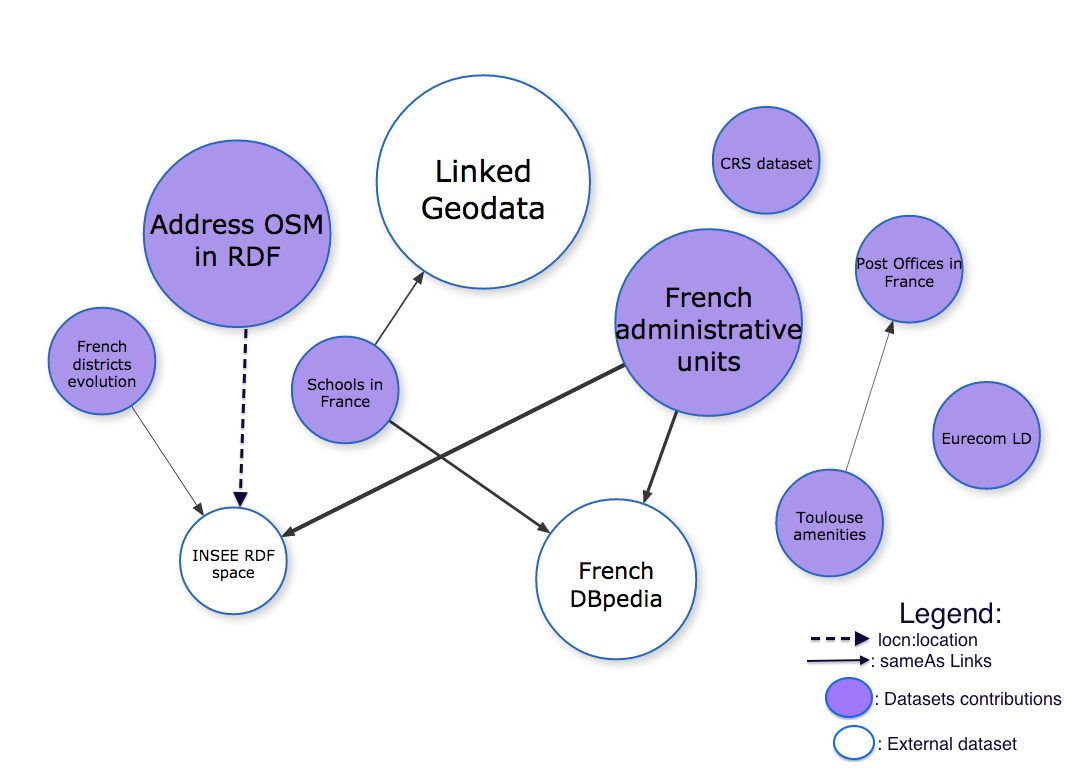
\includegraphics[width=\linewidth]{img/frenchCloud.png}
  
    \caption{French LOD Cloud based on the different datasets published in 4-5 stars. }
    \label{visuGraphModel}
  }
\end{figure}